% RuleDep Method Overview - Three-column layout with algorithm in middle
\documentclass[tikz,border=2mm]{standalone}
\usepackage{amsmath}
\usepackage{amssymb}
\usepackage{tikz}
\usepackage{algorithm}
\usepackage{algorithmic}
\usetikzlibrary{shapes.geometric, arrows.meta, positioning, fit, backgrounds, calc}

\definecolor{lightblue}{RGB}{173,216,230}
\definecolor{lightgreen}{RGB}{144,238,144}
\definecolor{lightyellow}{RGB}{255,250,205}
\definecolor{lightred}{RGB}{255,182,193}
\definecolor{lightgray}{RGB}{240,240,240}
\definecolor{alphablue}{RGB}{47,102,194}
\definecolor{betared}{RGB}{196,64,64}

\begin{document}

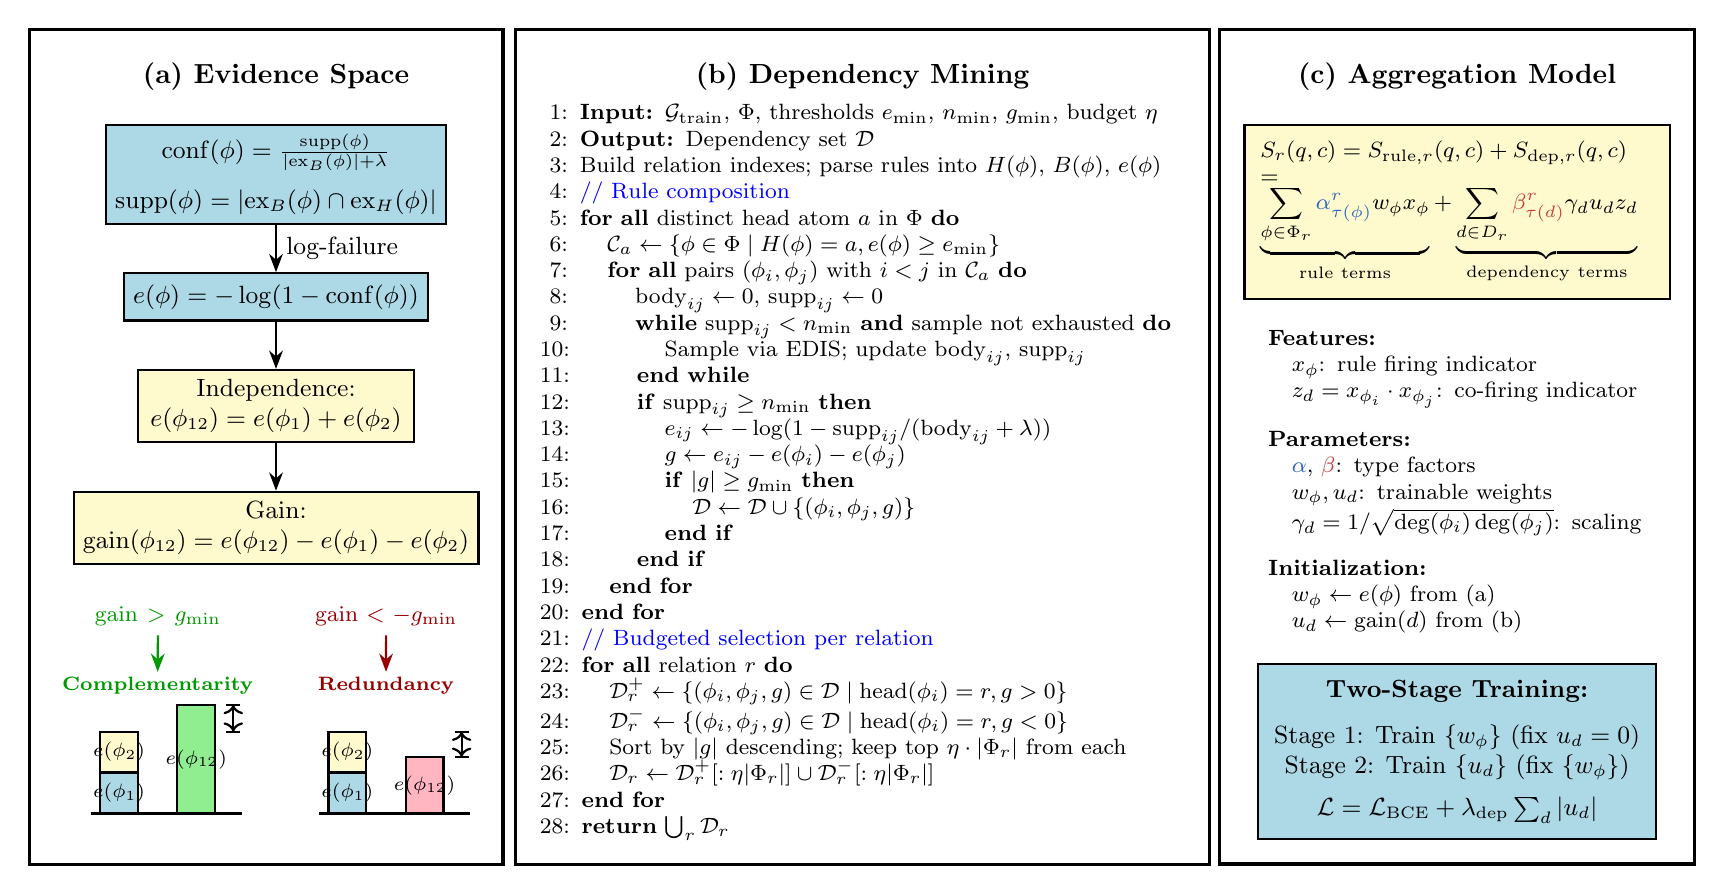
\begin{tikzpicture}[
    node distance=0.3cm,
    box/.style={rectangle, draw, thick, minimum width=2.8cm, minimum height=0.6cm, align=center, font=\small},
    title/.style={font=\bfseries\normalsize},
    arrow/.style={-Stealth, thick},
    formula/.style={font=\footnotesize, align=left},
    section/.style={rectangle, draw=black, very thick, inner sep=3mm}
]

% ============ (a) Evidence Transformation (3 units) ============
\node[title] (title-a) at (0, 0) {(a) Evidence Space};

% Confidence to evidence transformation
\node[box, fill=lightblue, below=0.3cm of title-a] (conf) {
    $\mathrm{conf}(\phi) = \frac{\mathrm{supp}(\phi)}{|\mathrm{ex}_B(\phi)|+\lambda}$
    \\[2mm]
    $\mathrm{supp}(\phi) = |\mathrm{ex}_B(\phi) \cap \mathrm{ex}_H(\phi)|$
};


% \node[formula, below=0.3cm of title-a, text width=5cm, draw, thick, fill=lightyellow, inner sep=3mm] 


\node[box, fill=lightblue, below=0.6cm of conf, minimum width=3.5cm] (evidence) {$e(\phi) = -\log(1-\mathrm{conf}(\phi))$};
\draw[arrow] (conf) -- (evidence) node[midway, right, font=\small] {log-failure};

% Independence baseline
\node[box, fill=lightyellow, below=0.6cm of evidence, minimum width=3.5cm] (indep) {Independence:\\$e(\phi_{12}) = e(\phi_1) + e(\phi_2)$};

% Gain definition
\node[box, fill=lightyellow, below=0.6cm of indep, minimum width=3.5cm] (gain) {Gain:\\$\operatorname{gain}(\phi_{12}) = e(\phi_{12}) - e(\phi_1) - e(\phi_2)$};
\draw[arrow] (evidence) -- (indep);
\draw[arrow] (indep) -- (gain);

% Gain interpretation
\node[formula, below=0.4cm of gain, xshift=-1.5cm, text width=2.1cm, align=center, text=green!60!black] (interp-left) {
    $\operatorname{gain} > g_{\min}$
};
\node[formula, text width=2.1cm, align=center, text=red!60!black, right=0.55cm of interp-left] (interp-right) {
    $\operatorname{gain} < -g_{\min}$
};

% Stacked-bar intuition for complementarity and redundancy
\node[below=0.15cm of interp-left.south east, minimum width=5.0cm, minimum height=2.45cm, inner sep=2mm] (note-a) {};

% Left mini-chart: Complementarity
\coordinate (c-base) at ($(note-a.south west)+(0.60cm,0.35cm)$);
\draw[thick] ($(c-base)+(-0.12cm,0)$) -- ($(c-base)+(1.80cm,0)$);
\fill[lightblue, draw=black, thick] ($(c-base)+(0.00cm,0.00cm)$) rectangle ($(c-base)+(0.48cm,0.52cm)$);
\fill[lightyellow, draw=black, thick] ($(c-base)+(0.00cm,0.52cm)$) rectangle ($(c-base)+(0.48cm,1.04cm)$);
\fill[lightgreen, draw=black, thick] ($(c-base)+(0.98cm,0.00cm)$) rectangle ($(c-base)+(1.46cm,1.38cm)$);
\draw[thick] ($(c-base)+(1.60cm,1.04cm)$) -- ($(c-base)+(1.78cm,1.04cm)$);
\draw[thick] ($(c-base)+(1.60cm,1.38cm)$) -- ($(c-base)+(1.78cm,1.38cm)$);
\draw[thick,<->] ($(c-base)+(1.69cm,1.04cm)$) -- ($(c-base)+(1.69cm,1.38cm)$);
\node[font=\scriptsize, align=center] at ($(c-base)+(0.24cm,0.26cm)$) {$e(\phi_1)$};
\node[font=\scriptsize, align=center] at ($(c-base)+(0.24cm,0.78cm)$) {$e(\phi_2)$};
\node[font=\scriptsize, align=center] at ($(c-base)+(1.22cm,0.69cm)$) {$e(\phi_{12})$};
\node[font=\scriptsize\bfseries, text=green!60!black, align=center] at ($(c-base)+(0.73cm,1.62cm)$) {Complementarity};
\draw[arrow, green!60!black] (interp-left.south) -- ($(c-base)+(0.73cm,1.8cm)$);

% Right mini-chart: Redundancy
\coordinate (r-base) at ($(note-a.south west)+(3.5cm,0.35cm)$);
\draw[thick] ($(r-base)+(-0.12cm,0)$) -- ($(r-base)+(1.80cm,0)$);
\fill[lightblue, draw=black, thick] ($(r-base)+(0.00cm,0.00cm)$) rectangle ($(r-base)+(0.48cm,0.52cm)$);
\fill[lightyellow, draw=black, thick] ($(r-base)+(0.00cm,0.52cm)$) rectangle ($(r-base)+(0.48cm,1.04cm)$);
\fill[lightred, draw=black, thick] ($(r-base)+(0.98cm,0.00cm)$) rectangle ($(r-base)+(1.46cm,0.72cm)$);
\draw[thick] ($(r-base)+(1.60cm,0.72cm)$) -- ($(r-base)+(1.78cm,0.72cm)$);
\draw[thick] ($(r-base)+(1.60cm,1.04cm)$) -- ($(r-base)+(1.78cm,1.04cm)$);
\draw[thick,<->] ($(r-base)+(1.69cm,0.72cm)$) -- ($(r-base)+(1.69cm,1.04cm)$);
\node[font=\scriptsize, align=center] at ($(r-base)+(0.24cm,0.26cm)$) {$e(\phi_1)$};
\node[font=\scriptsize, align=center] at ($(r-base)+(0.24cm,0.78cm)$) {$e(\phi_2)$};
\node[font=\scriptsize, align=center] at ($(r-base)+(1.22cm,0.36cm)$) {$e(\phi_{12})$};
\node[font=\scriptsize\bfseries, text=red!60!black, align=center] at ($(r-base)+(0.73cm,1.62cm)$) {Redundancy};
\draw[arrow, red!60!black] (interp-right.south) -- ($(r-base)+(0.73cm,1.8cm)$);

% Section box
\begin{scope}[on background layer]
\node[section, fit=(title-a)(conf)(evidence)(indep)(gain)(interp-left)(interp-right)(note-a)] (sec-a) {};
\end{scope}

% ============ (b) Dependency Mining Algorithm (5 units) ============
\node[title] (title-b) at (7.45, 0) {(b) Dependency Mining};

% Algorithm box
\node[below=-0.15cm of title-b, text width=8.2cm, font=\footnotesize, inner sep=0mm] (algo) {
\begin{algorithmic}[1]
\STATE \textbf{Input:} $\mathcal{G}_{\text{train}}$, $\Phi$, thresholds $e_{\min}$, $n_{\min}$, $g_{\min}$, budget $\eta$
\STATE \textbf{Output:} Dependency set $\mathcal{D}$
\STATE Build relation indexes; parse rules into $H(\phi)$, $B(\phi)$, $e(\phi)$
\STATE \textcolor{blue}{// Rule composition}
\FORALL{distinct head atom $a$ in $\Phi$}
    \STATE $\mathcal{C}_a \leftarrow \{\phi \in \Phi \mid H(\phi)=a, e(\phi) \ge e_{\min}\}$
    \FORALL{pairs $(\phi_i,\phi_j)$ with $i<j$ in $\mathcal{C}_a$}
        \STATE $\mathrm{body}_{ij} \leftarrow 0$, $\mathrm{supp}_{ij} \leftarrow 0$
        \WHILE{$\mathrm{supp}_{ij} < n_{\min}$ \textbf{and} sample not exhausted}
            \STATE Sample via EDIS; update $\mathrm{body}_{ij}$, $\mathrm{supp}_{ij}$
        \ENDWHILE
        \IF{$\mathrm{supp}_{ij} \ge n_{\min}$}
            \STATE $e_{ij} \leftarrow -\log(1-\mathrm{supp}_{ij}/(\mathrm{body}_{ij}+\lambda))$
            \STATE $g \leftarrow e_{ij} - e(\phi_i) - e(\phi_j)$
            \IF{$|g| \ge g_{\min}$}
                \STATE $\mathcal{D} \leftarrow \mathcal{D} \cup \{(\phi_i,\phi_j,g)\}$
            \ENDIF
        \ENDIF
    \ENDFOR
\ENDFOR
\STATE \textcolor{blue}{// Budgeted selection per relation}
\FORALL{relation $r$}
    \STATE $\mathcal{D}_r^{+} \leftarrow \{(\phi_i,\phi_j,g) \in \mathcal{D} \mid \text{head}(\phi_i)=r, g > 0\}$
    \STATE $\mathcal{D}_r^{-} \leftarrow \{(\phi_i,\phi_j,g) \in \mathcal{D} \mid \text{head}(\phi_i)=r, g < 0\}$
    \STATE Sort by $|g|$ descending; keep top $\eta \cdot |\Phi_r|$ from each
    \STATE $\mathcal{D}_r \leftarrow \mathcal{D}_r^{+}[:\eta|\Phi_r|] \cup \mathcal{D}_r^{-}[:\eta|\Phi_r|]$
\ENDFOR
\STATE \textbf{return} $\bigcup_r \mathcal{D}_r$
\end{algorithmic}
};

% Section box
\begin{scope}[on background layer]
\node[section, fit=(title-b)(algo), inner sep=3mm] (sec-b) {};
\end{scope}

% ============ (c) Aggregation Model (4 units) ============
\node[title] (title-c) at (15, 0) {(c) Aggregation Model};

% Model formula
\node[formula, below=0.3cm of title-c, text width=5cm, draw, thick, fill=lightyellow, inner sep=2mm] (model) {
    $S_r(q,c) = S_{\text{rule},r}(q,c) + S_{\text{dep},r}(q,c)$\\
    $= \underbrace{\sum_{\phi \in \Phi_r} \textcolor{alphablue}{\alpha_{\tau(\phi)}^r} w_\phi x_\phi}_{\text{rule terms}} + \underbrace{\sum_{d \in D_r} \textcolor{betared}{\beta_{\tau(d)}^r} \gamma_d u_d z_d}_{\text{dependency terms}}$
};

% =\sum_{\phi\in\Phi_r} \alpha^r_{\tau(\phi)} w_{\phi}x_{\phi}(q,c)
% +\sum_{d\in\mathcal{D}_r} \beta^r_{\tau(d)}\gamma_d u_d z_d(q,c)

% Annotations
\node[formula, below=0.25cm of model, text width=4.8cm] (annot1) {
    \textbf{Features:}\\
    \hspace{3mm}$x_\phi$: rule firing indicator\\
    \hspace{3mm}$z_d = x_{\phi_i} \cdot x_{\phi_j}$: co-firing indicator
};

\node[formula, below=0.05cm of annot1, text width=4.8cm] (annot2) {
    \textbf{Parameters:}\\
    \hspace{3mm}\textcolor{alphablue}{$\alpha$}, \textcolor{betared}{$\beta$}: type factors\\
    \hspace{3mm}$w_\phi, u_d$: trainable weights\\
    \hspace{3mm}$\gamma_d = 1/\sqrt{\deg(\phi_i)\deg(\phi_j)}$: scaling
};

\node[formula, below=0.05cm of annot2, text width=4.8cm] (annot3) {
    \textbf{Initialization:}\\
    \hspace{3mm}$w_\phi \leftarrow e(\phi)$ from (a)\\
    \hspace{3mm}$u_d \leftarrow \operatorname{gain}(d)$ from (b)
};

% Training box
\node[box, fill=lightblue, below=0.25cm of annot3, minimum width=4.8cm, minimum height=1.5cm, inner sep=2mm] (training) {
    \textbf{Two-Stage Training:}\\[2mm]
    Stage 1: Train $\{w_\phi\}$ (fix $u_d=0$)\\
    Stage 2: Train $\{u_d\}$ (fix $\{w_\phi\}$)\\[1.5mm]
    $\mathcal{L} = \mathcal{L}_{\text{BCE}} + \lambda_{\text{dep}} \sum_{d} |u_d|$
};

% Section box
\begin{scope}[on background layer]
\node[section, fit=(title-c)(model)(annot1)(annot2)(annot3)(training)] (sec-c) {};
\end{scope}

\end{tikzpicture}

\end{document}